\input{/Users/oscar/Documents/LaTeX_Templates/HW.tex}
% \input{/home/oscar/Documents/LaTeX_Templates/HW.tex}

\title{Notes of Probability Theory}
\date{\today}
\author{董海辰 518030910417\\{\normalsize with help from 毛昕渝}}

\begin{document}
\maketitle

\begin{thm}{Definitions}{}
    \begin{itemize}
        \item From digits(tree paths) to intervals.
        \item normal numbers
    \item A subset $A$ of $\mathbb{R} $ is \textit{negligible} if $\forall \varepsilon >0$, there exists a finite or countable collection $I_1, I_2, \cdots $ of (possibly overlapping) intervals satisfying: $A \subset \bigcup_k I_k$ and $\sum _k|I_k| < \varepsilon $.
    \end{itemize}
\end{thm}

Every path of the binary tree is a real number in binary form.

Two numbers are equal if there are no paths between: e.g. $0.010000\cdots $ and $0.0011111\cdots $.

$P(\omega : d(i,\omega ) = u_i, i = 1,2,\cdots ,n) = 2^{-n}$.

\begin{figure}[h!]
    \centering
    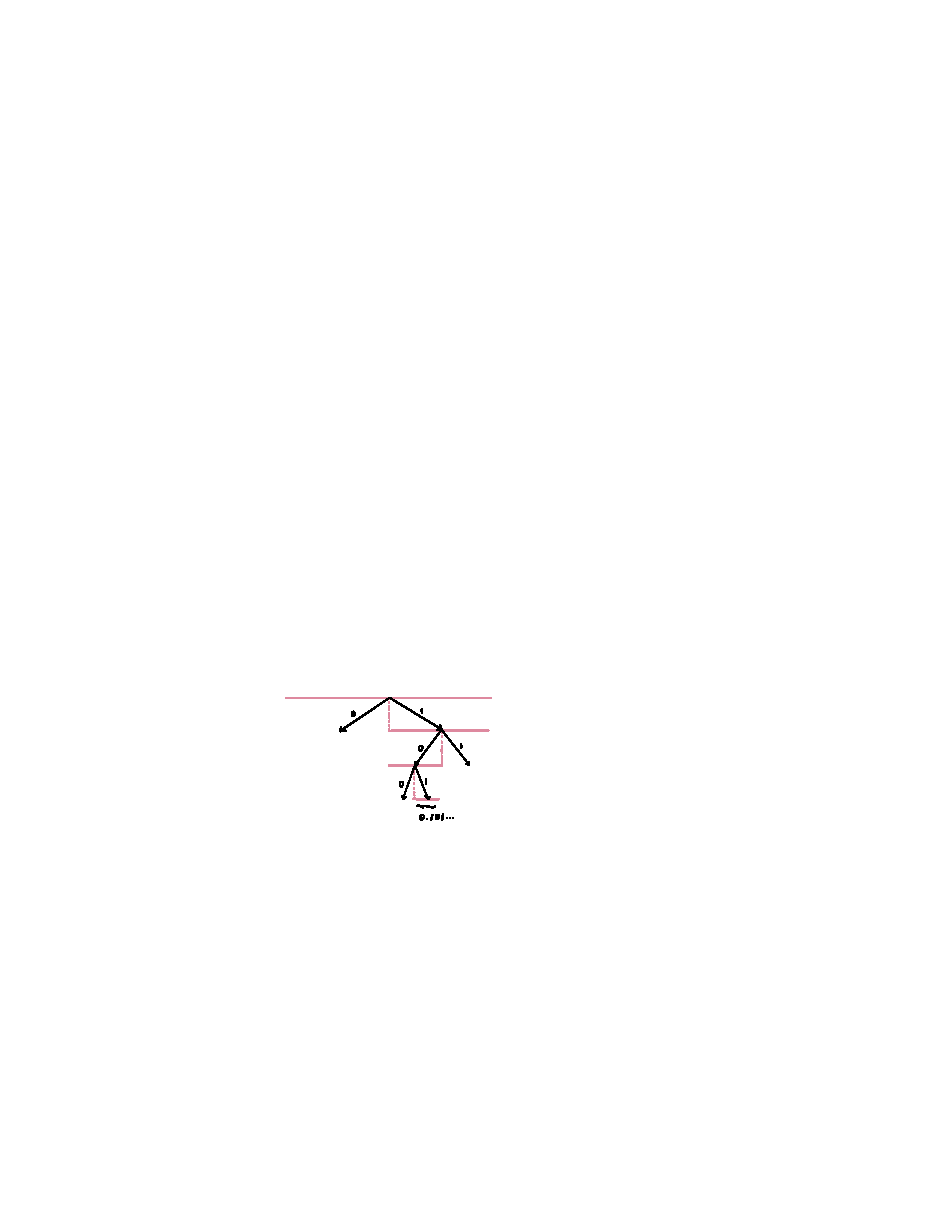
\includegraphics[width=0.45\textwidth]{w1fig.pdf}
    \caption{digits to intervals}
\end{figure}

\begin{thm}{Weak Law of Large Numbers}{}
    \begin{align*}
        \forall  \varepsilon >0, \lim_{n\to \infty}P(\omega \in \Omega : |\frac{\sum_{i=1}^n d_i(\omega)}{n} - \frac{1}{2}| \ge \varepsilon ) = 0
    .\end{align*}
\end{thm}

For each $n$, the $P$ can be calculated by summing up the lengths of every interval that meet the condition.

Let $r_i(\omega ) = 2d_i(\omega ) - 1$.
\begin{qte}
    $r_i(\omega )$ are Orthonomal basis, i.e.
    \begin{align*}
        \int_\Omega r_i(\omega )r_j(\omega ) \mathrm{d} w = \delta_{i,j}
    .\end{align*}

    If $i \neq j$, say $i < j$, there are equal number if intervals that $r_j(\omega ) = 1$ and $r_j(\omega ) = -1$, resulting in sum $0$.
\end{qte}

Let $S_n(\omega ) = \sum_{i=1}^n r_i(\omega )$,
\begin{align*}
    P[\omega : |S_n(\omega )| \ge 2n\varepsilon ] &\le \frac{1}{4n^2\varepsilon ^2} \int_0^1 S_n^2(\omega )\dd\omega \\
    &= \frac{1}{4n^2\varepsilon ^2}n = \frac{1}{4n\varepsilon ^2} \to  0
.\end{align*}

\begin{qte}
    Here applied the Chebyshev's Inequality:
    \begin{align*}
        P[|X - E(X)| \ge b] \le \frac{Var(X)}{b^2}
    .\end{align*}

    And note that $r_i(\omega )$ are orthogonal,
    \begin{align*}
        Var(S_n(\omega )) = \int_\Omega S_n^2(\omega )\dd\omega = \int_\Omega (\sum r_i(\omega ))^2 \dd\omega = \int_\Omega r_i^2(\omega )\dd\omega  = n
    .\end{align*}
\end{qte}

\begin{thm}{Strong Law of Large Numbers}{}
    Borel's Normal Number Theorem

    The complement of the set of normal numbers to base $2$ is uncountable but negligible.
    \begin{align*}
        \mathcal{N} = \{\omega : \lim_{n\to \infty} \frac{S_n(\omega )}{n} = 0\}
    .\end{align*}

    $\Omega \backslash \mathcal{N}$ is uncountable, but
    \begin{align*}
        \forall \varepsilon > 0, \exists I_1, I_2, \cdots I_n \cdots , \Omega \backslash \mathcal{N} \subseteq \bigcup_i I_i, \sum_i |I_i| < \varepsilon 
    .\end{align*}
\end{thm}

Let $A_n = [\omega :|\frac{S_n(\omega )}{n}\ge \varepsilon _n]$ where $e_n \to 0$. Thus 
\begin{align*}
    \Omega \backslash \mathcal{N} = \lim_{m\to \infty}\bigcup _{n=m}^\infty A_n
.\end{align*}

\begin{qte}{}{}
    We have
    \begin{align*}
        \omega \in \mathcal{N} \iff \forall \varepsilon > 0, \exists m > 0, \forall n>m,|\frac{S_n}{n}| < \varepsilon \iff \omega \not\in \bigcup_{n=m}^\infty A_n
    .\end{align*}

    And show $|\Omega \backslash \mathcal{N}| < \sum_{n=m}^\infty |A_n| < \varepsilon_n $
\end{qte}

\begin{align*}
    P[\omega : |\frac{S_n(\omega )}{n}| \ge \varepsilon_n ] &\le \frac{1}{n^4\varepsilon_n ^4} \int_0^1 S_n^4(\omega )\dd\omega  \\
                                                          &=\frac{n+3n(n-1)}{n^4\varepsilon_n ^4} \le \frac{3}{n^2\varepsilon_n ^4}
.\end{align*}

\begin{qte}
    Let $1_{A_n}(\omega ) = 1$ for all $\omega \in A_n$ and be $0$ otherwise.

    Then $\forall \omega \in \Omega , 1_{A_n}(\omega ) \le \frac{S_n^4(\omega )}{n^4 \varepsilon _n^4}$. We can get
    \begin{align*}
        P[\omega :\omega \in A_n] = \int_\Omega 1_{A_n}(\omega ) \dd \omega \le \int_\Omega \frac{S^4_n(\omega) }{n^4\varepsilon _n^4} \dd \omega 
    .\end{align*}

    Similarly, $S^4_n(\omega ) = (\sum _{i=1}^n r_i(\omega ))^4$. Terms with non-zero values are:
    \begin{itemize}
        \item $r_i^4(\omega ) = 1$
        \item $r_i^2(\omega ) r_j^2(\omega ) = 1$
    \end{itemize}
    With sum $\binom n 1 + \binom n 2 \cdot \binom 4 2 = n + 3n(n-1)$.
\end{qte}

$\{e_n\}$ is a sequence with $\lim_{n\to \infty}e_n = 0$, we can let $e_n = n^{-\frac{1}{8}} $, and 
\begin{align*}
    \sum_{n=1}^\infty |A_n| \le  \sum_{n=1}^\infty\frac{3}{n^{\frac{3}{2}}}
\end{align*}
, which is convergent. And intervals of $\bigcup_{n=m}^\infty A_n$ is countable. Thus
\begin{align*}
    \forall \varepsilon > 0, \exists m > 0,  \Omega \backslash \mathcal{N} \subseteq \bigcup_{n=m}^\infty A_n, \sum _{n=m}^\infty |A_n| < \varepsilon 
.\end{align*}

\begin{qte}{}{}
    If we use the inequality in proof of WLLN: $P[\omega : \omega \in A_n] \le \frac{1}{n \varepsilon_n ^2}$. In this case, whatever $\{e_n\} $ we choose, the sum will never be convergent.
\end{qte}

\end{document}
